\section*{35. Интегральный вид уравнений Максвелла и граничные условия для
магнитного поля при наличии сред.}

\begin{minipage}[c]{0.4\textwidth} % Левая часть: изображение
    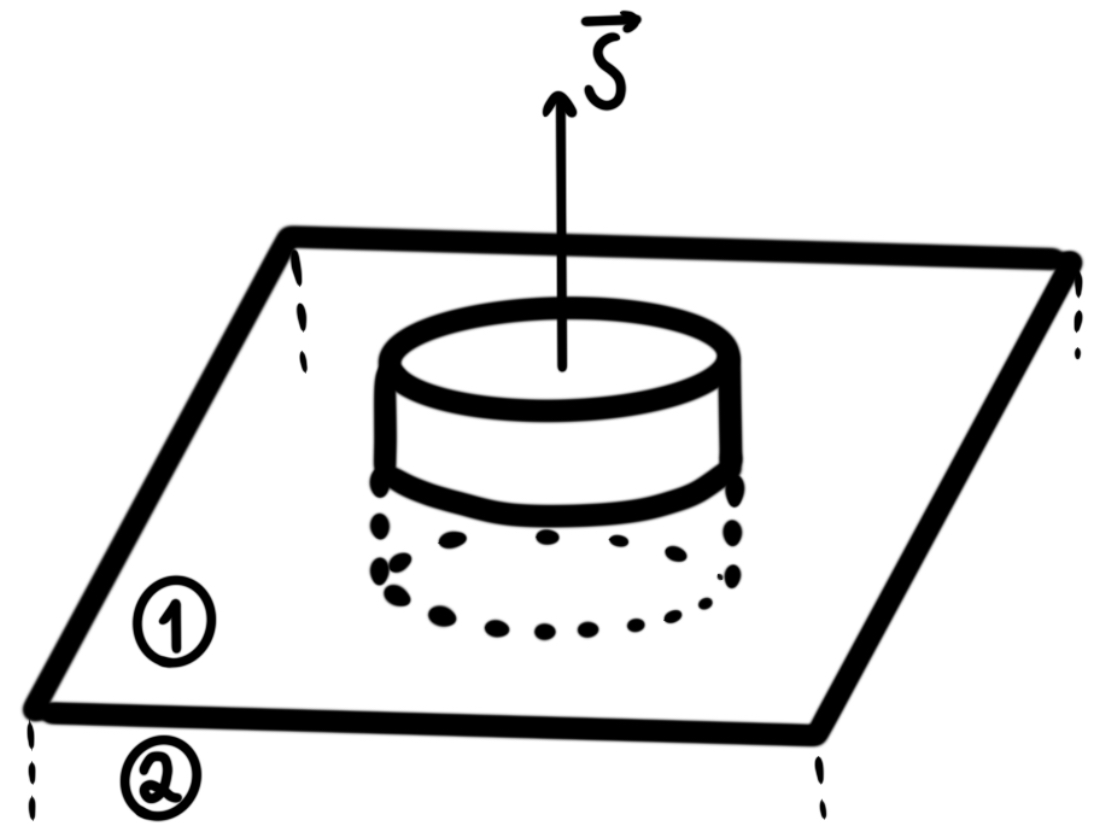
\includegraphics[width=\textwidth]{im/73.png} % Ваше изображение
\end{minipage}%
\hfill
\begin{minipage}[c]{0.7\textwidth} % Правая часть: текст
    \begin{gather*}
        \mathrm{div}\vec{B}=0 \\
        \downarrow \\
        \oiint \vec{B}d\vec{S}=0 
    \end{gather*}
\end{minipage}

\[
B_{1n}|\cdot S-B_{2n}|\cdot S=0 \Rightarrow \boxed{B_n|-\text{непр.}}
\]

\begin{minipage}[c]{0.4\textwidth} % Левая часть: изображение
    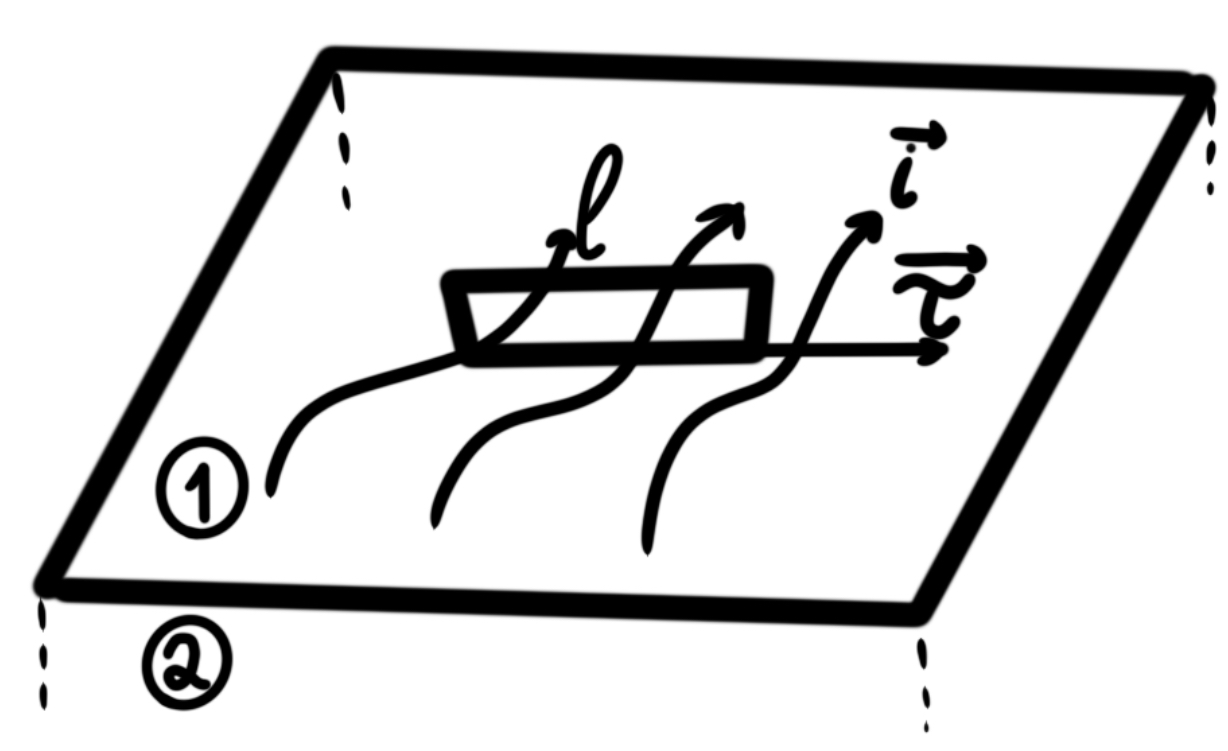
\includegraphics[width=\textwidth]{im/74.png} % Ваше изображение
\end{minipage}%
\hfill
\begin{minipage}[c]{0.6\textwidth} % Правая часть: текст
    \begin{gather*}
        \mathrm{rot}\vec{H}=\frac{4\pi}{c}\vec{j}  \\
        \downarrow \\
        \oint \vec{H}d\vec{l}=\frac{4\pi}{c} 
    \end{gather*}
\end{minipage}

\[
H_{1\tau}|\cdot l -H_{2\tau}|\cdot l=\frac{4\pi}{c}il \Rightarrow \boxed{H_{1\tau}|-H_{2\tau}|=\frac{4\pi}{c}i } 
\]